\section{Part B}
\subsection{Technical Discussion}
\subsubsection{Histogram Processing}
The histogram of a digital image with intensity levels in the range [$0, L - 1$] is a discrete function $h(r_k) = n_k$, where $r_k$ is the $k$th intensity value and $n_k$ is the number of pixels in the image with intensity $r_k$. It is common practice to normalize a histogram by dividing each of its components by the total number of pixels in the image, denoted by the product $MN$, where, as usual, $M$ and $N$ are the row and column dimensions of the image. Thus, a normalized histogram is given by $p(r_k) = n_k/MN$, for $k = 0, 1, 2, ..., L-1$. Loosely speaking, $p(r_k)$ is an estimate of the probability of occurrence of intensity level $r_k$ in an image. The sum of all components of a normalized histogram is equal to 1.
\subsubsection{Histogram Equalization}
As we know, if we view input intensities $r$ and output intensity $s$ as random variables and their histograms as probability density functions(pdf) $p_r(r)$ and $p_s(s)$.\\
if $p_r(r)$ and $T(r)$ are known and $T(r)$ is continuous and differentiable, then,
$$ p_s(s) = p_r(r)\frac{1}{\left| \frac{ds}{dr} \right|} = p_r(r)\left| \frac{dr}{ds} \right| $$ 
Cumulative distribution function of a random Variable:
$$s = T(r) = (L - 1)\int_0^r p_r(w)dw$$
To fund $p_s(s)$ we have to compute
$$ \frac{ds}{dr} = \frac{dT(r)}{dr} = (L - 1)\frac{d}{dr}\int_0^r p_r(w)dw = (L - 1)p_r(r) $$
Substituting this result:
$$ \frac{ds}{dr} = (L - 1)p_r(r) $$
to 
$$ p_s(s) = p_r(r)\left| \frac{dr}{ds} \right| $$
yields
$$p_s(s) = p_r(r)\left| \frac{1}{(L - 1)p_r(r)} = \frac{1}{L - 1} \right|, 0 \leq s \leq L - 1 $$
The formula for histogram equalisation in the discrete case is given
$$ s_k = T(r_k) = (L - 1)\sum_{j = 0}^k p_r(r_j) = \frac{L - 1}{MN}\sum_{j = 0}^{k} n_j $$
\subsection{Discussion of Results}
\subsubsection{Computing the histogram of an image}
The original image is shown in Figure \ref{fig:hisoriginal}
\begin{figure}[h]
	\centering
	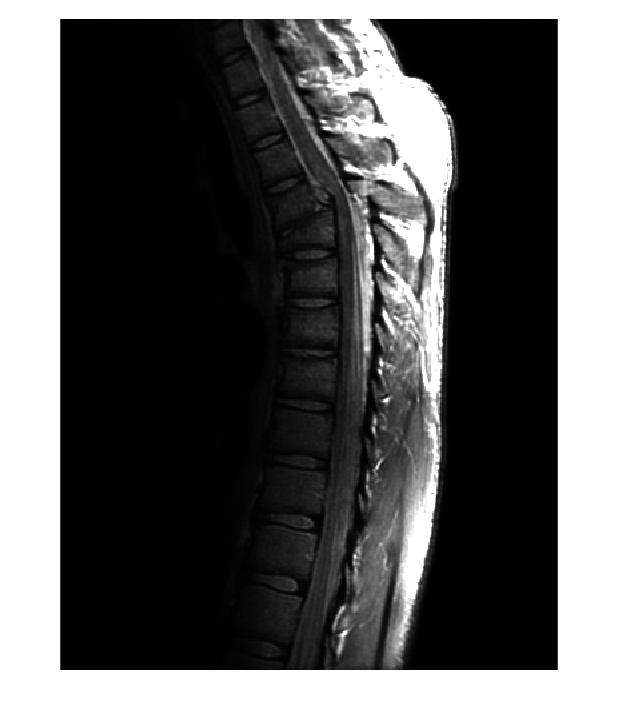
\includegraphics[scale=0.2]{0308}
	\caption{Original Image}
	\label{fig:hisoriginal}
\end{figure}
To get the histogram of given image, we need to iterate all pixel values of the image and get the frequency of each intencity. Figure \ref{fig:hishist1} shows the output histogram of Figure \ref{fig:hisoriginal} after normalisation. We can note that most pixel values are on the dark side.
\begin{figure}[h]
	\centering
	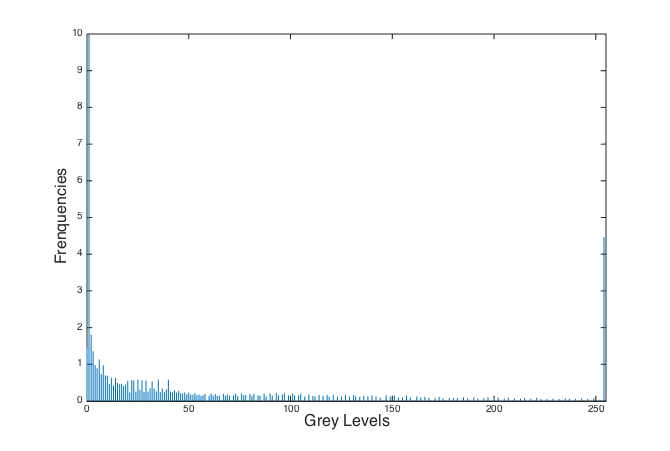
\includegraphics[scale=0.4]{historg}
	\caption{Histogram of Figure \ref{fig:hisoriginal}}
	\label{fig:hishist1}
\end{figure}
\subsubsection{Implemention of histogram equalization}
To perform histogram equalization on given image, we could use the formula for histogram equalization in the discrete case
$$ s_k = T(r_k) = \frac{L - 1}{MN}\sum_{j = 0}^{k} n_j $$
\\[10cm]
\begin{figure}[h]
	\centering
	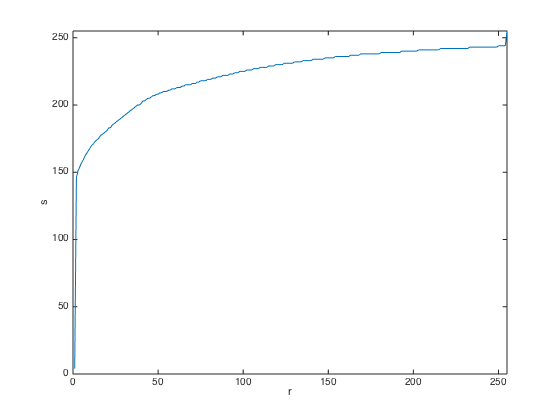
\includegraphics[scale=0.4]{hetrans}
	\caption{Transformation function}
	\label{fig:hetrans}
\end{figure}

Figure \ref{fig:hetrans} shows the transformation function. Figure \ref{fig:histeq} shows the comparision between the original image and the image after histogram equalization. We can notice that the produced image is much lighter than original image and we could get more details on the darker side of the image. However, the background became too light after histogram equalization, which reduce the contrast of image. Figure \ref{fig:histnew} shows the histogram of the produced image. \\
\\
The reason of the background became too light can be described as follows. As we can see from the histogram of original image in Figure \ref{fig:hishist1}, most of the pixel values in orinal image are concentrated neat 0. According to the formula for histogram equalization in the discrete case
$ s_k = T(r_k) = \frac{L - 1}{MN}\sum_{j = 0}^{k} n_j $, if there are too many pixel values nears 0, then the output value $s$ will grow a lot for those input pixels with value near 0. As a result, the produced image have a washed-out appearance. 
\begin{figure}[h]
	\centering
	\subfloat[Subfigure 1 list of figures text][Original Image]{
		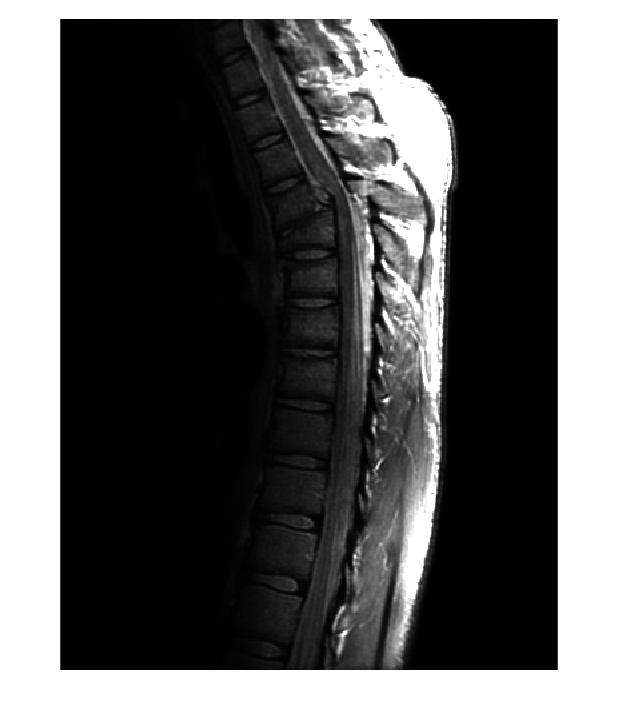
\includegraphics[width=0.2\textwidth]{0308}
		\label{fig:histeqsub1}}
	\subfloat[Subfigure 2 list of figures text][Image after histogram equalization]{
		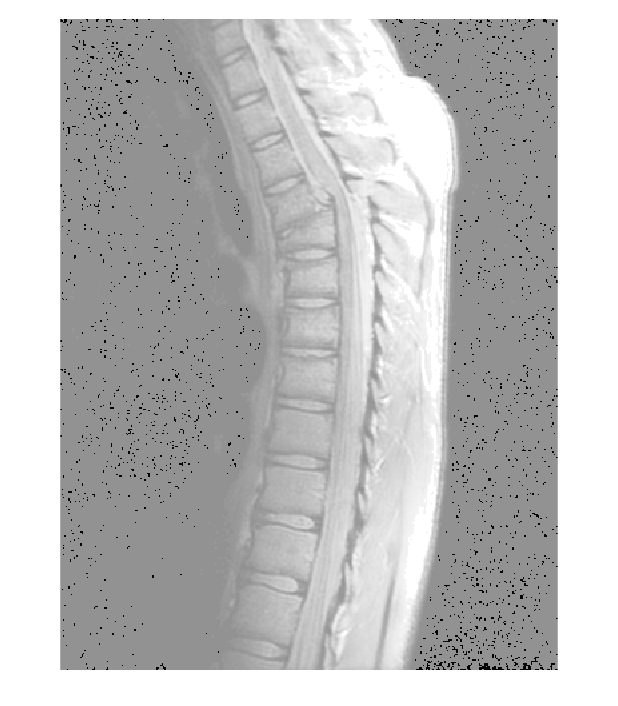
\includegraphics[width=0.2\textwidth]{histeq}
		\label{fig:histeqsub2}}
	\caption{Experiments results of histogram equalization}
	\label{fig:histeq}
\end{figure}

\begin{figure}[h]
	\centering
	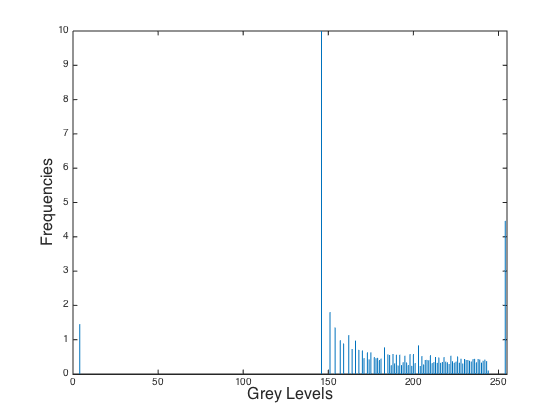
\includegraphics[scale=0.4]{histnew}
	\caption{Histogram of produced image}
	\label{fig:histnew}
\end{figure}
\newpage